\documentclass[11pt]{article}
\usepackage[textwidth=18.0cm, textheight=23.0cm, top=2.0cm]{geometry}
\usepackage{pst-all}
\usepackage{amssymb}
\usepackage{tikz}
\usepackage{underscore}\begin{document}
\pagestyle{empty}


ClassName: \underline{\textbf{Class_08.2bp-22}}
\par
BinSize: \underline{\textbf{100 × 100}}
\par
ReduceSize: \underline{\textbf{100 × 100}}
\par
TypeNum: \underline{\textbf{60}}
\par
Num: \underline{\textbf{60}}
\par
OutS: \underline{\textbf{170000}}
\par
InS: \underline{\textbf{140453}}
\par
Rate: \underline{\textbf{0.826}}
\par
UB: \underline{\textbf{17}}
\par
LB0: \underline{\textbf{16}}
\par
LB: \underline{\textbf{16}}
\par
LBWithCut: \underline{\textbf{16}}
\par
NodeCut: \underline{\textbf{0}}
\par
ExtendedNodeCnt: \underline{\textbf{1}}
\par
GenNodeCnt: \underline{\textbf{1}}
\par
PrimalNode: \underline{\textbf{7}}
\par
ColumnCount: \underline{\textbf{117}}
\par
TotalCutCount: \underline{\textbf{0}}
\par
RootCutCount: \underline{\textbf{0}}
\par
LPSolverCnt: \underline{\textbf{118}}
\par
PricingSolverCnt: \underline{\textbf{117}}
\par
BranchAndBoundNum: \underline{\textbf{1}}
\par
isOpt: \underline{\textbf{false}}
\par
TimeOnInitSolution: \underline{\textbf{600.000 s}}
\par
TimeOnPrimal: \underline{\textbf{828.299 s}}
\par
TimeOnPricing: \underline{\textbf{2999.522 s}}
\par
TimeOnRmp: \underline{\textbf{0.182 s}}
\par
TotalTime: \underline{\textbf{3599.996 s}}
\par
\newpage


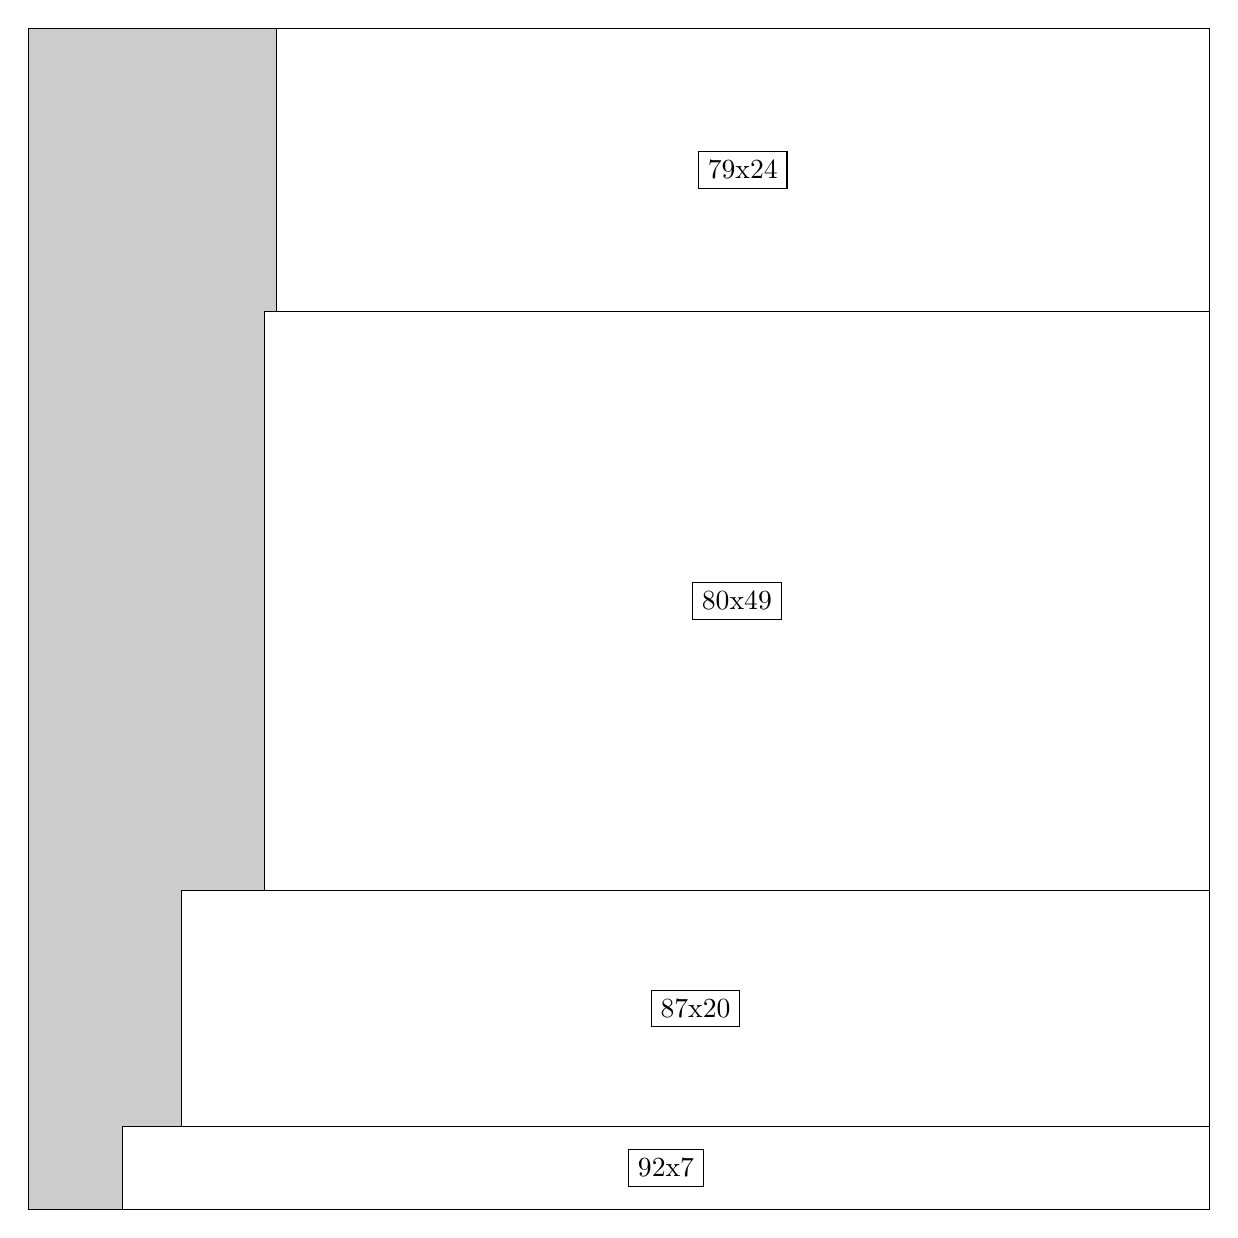
\begin{tikzpicture}[shorten >=1pt,scale=1.0,every node/.style={scale=1.0},->]
\tikzstyle{vertex}=[circle,fill=black!25,minimum size=14pt,inner sep=0pt]
\filldraw[fill=gray!40!white, draw=black] (0,0) rectangle (15.0,15.0);
\foreach \name/\x/\y/\w/\h in {92x7/1.2/0.0/13.799999999999999/1.05,87x20/1.95/1.05/13.049999999999999/3.0,80x49/3.0/4.05/12.0/7.35,79x24/3.15/11.4/11.85/3.5999999999999996}
\filldraw[fill=white!40!white, draw=black] (\x,\y) rectangle node[draw] (\name) {\name} ++(\w,\h);
\end{tikzpicture}


w =92 , h =7 , x =8 , y =0 , v =644
\par
w =87 , h =20 , x =13 , y =7 , v =1740
\par
w =80 , h =49 , x =20 , y =27 , v =3920
\par
w =79 , h =24 , x =21 , y =76 , v =1896
\par
\newpage


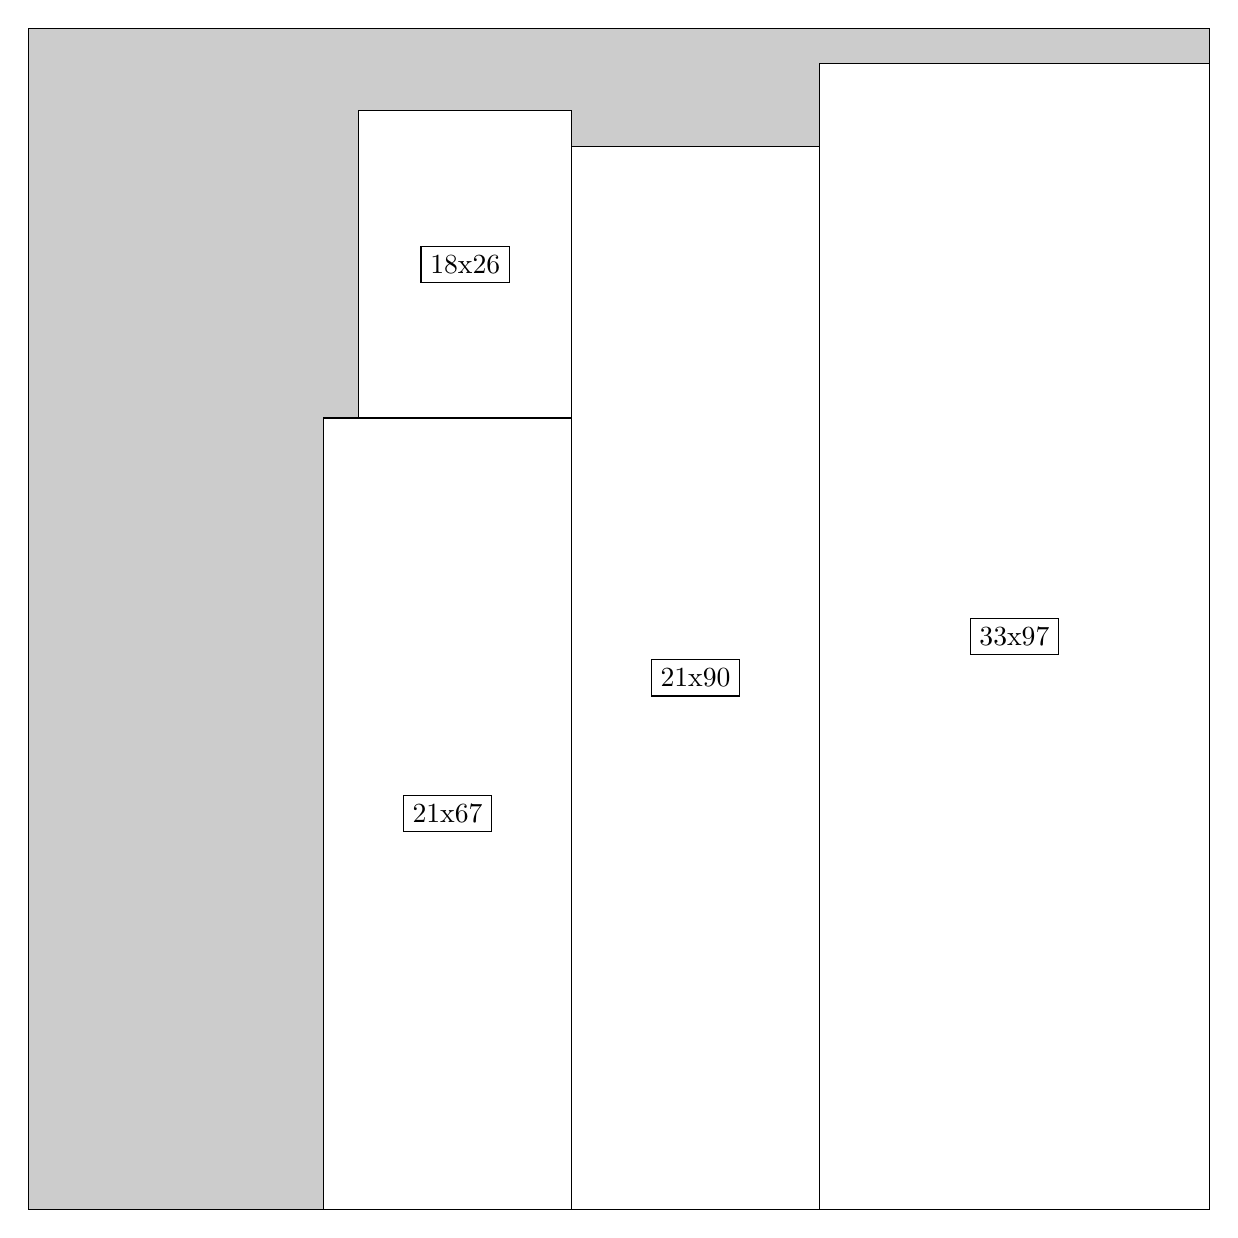
\begin{tikzpicture}[shorten >=1pt,scale=1.0,every node/.style={scale=1.0},->]
\tikzstyle{vertex}=[circle,fill=black!25,minimum size=14pt,inner sep=0pt]
\filldraw[fill=gray!40!white, draw=black] (0,0) rectangle (15.0,15.0);
\foreach \name/\x/\y/\w/\h in {33x97/10.049999999999999/0.0/4.95/14.549999999999999,21x90/6.8999999999999995/0.0/3.15/13.5,21x67/3.75/0.0/3.15/10.049999999999999,18x26/4.2/10.049999999999999/2.6999999999999997/3.9}
\filldraw[fill=white!40!white, draw=black] (\x,\y) rectangle node[draw] (\name) {\name} ++(\w,\h);
\end{tikzpicture}


w =33 , h =97 , x =67 , y =0 , v =3201
\par
w =21 , h =90 , x =46 , y =0 , v =1890
\par
w =21 , h =67 , x =25 , y =0 , v =1407
\par
w =18 , h =26 , x =28 , y =67 , v =468
\par
\newpage


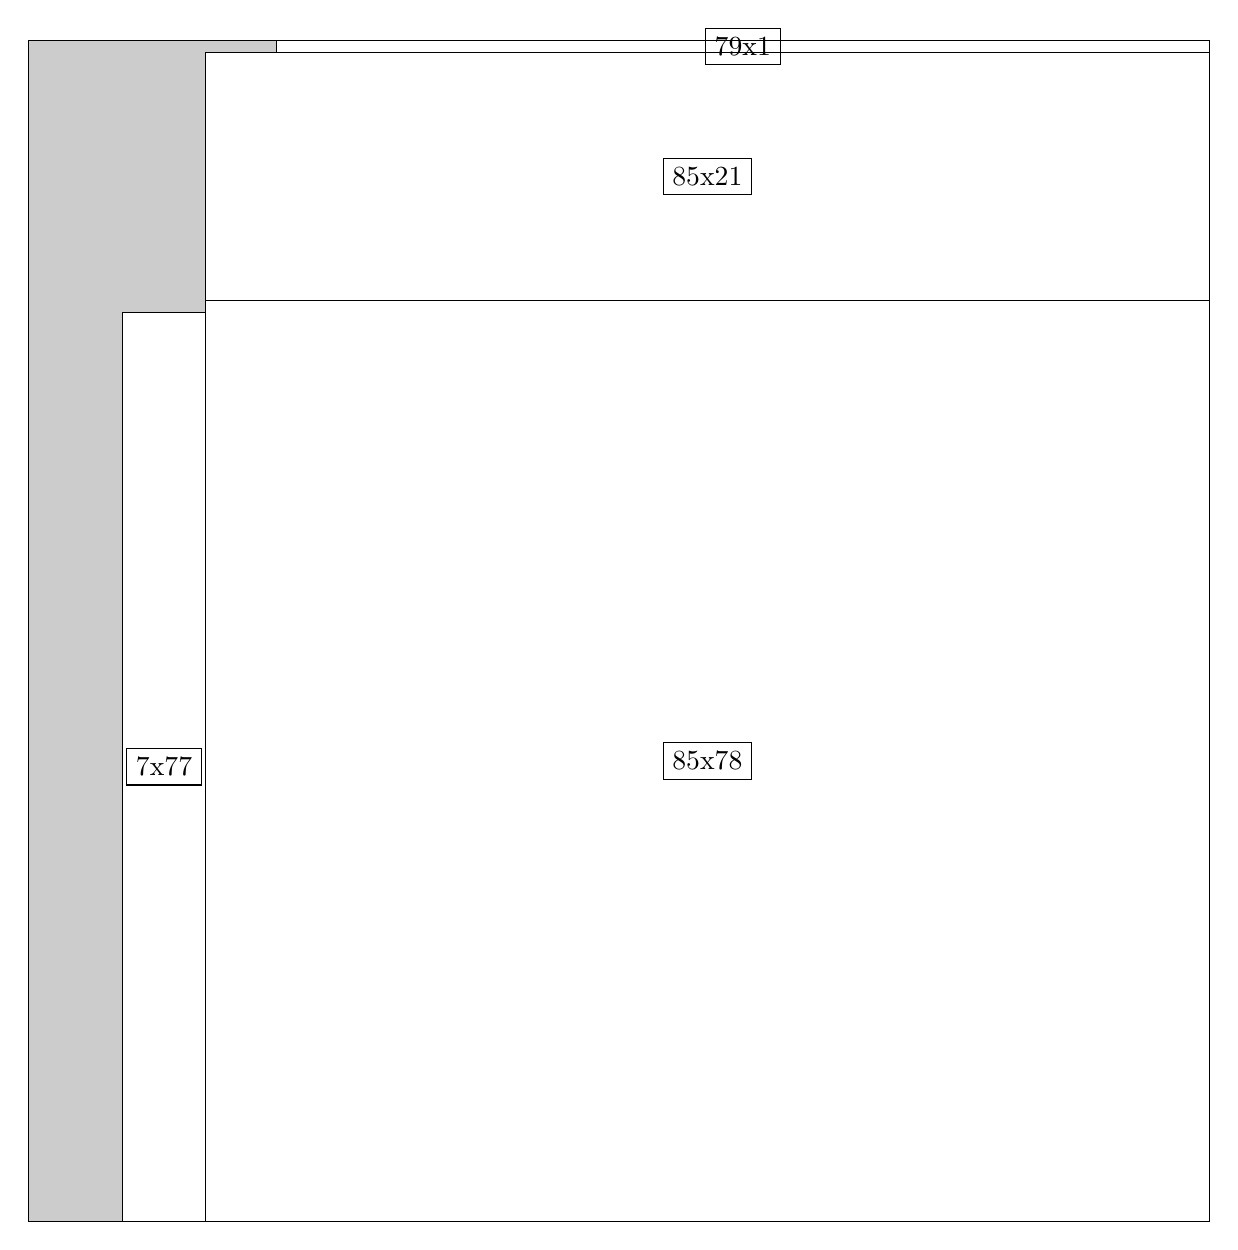
\begin{tikzpicture}[shorten >=1pt,scale=1.0,every node/.style={scale=1.0},->]
\tikzstyle{vertex}=[circle,fill=black!25,minimum size=14pt,inner sep=0pt]
\filldraw[fill=gray!40!white, draw=black] (0,0) rectangle (15.0,15.0);
\foreach \name/\x/\y/\w/\h in {85x78/2.25/0.0/12.75/11.7,85x21/2.25/11.7/12.75/3.15,79x1/3.15/14.85/11.85/0.15,7x77/1.2/0.0/1.05/11.549999999999999}
\filldraw[fill=white!40!white, draw=black] (\x,\y) rectangle node[draw] (\name) {\name} ++(\w,\h);
\end{tikzpicture}


w =85 , h =78 , x =15 , y =0 , v =6630
\par
w =85 , h =21 , x =15 , y =78 , v =1785
\par
w =79 , h =1 , x =21 , y =99 , v =79
\par
w =7 , h =77 , x =8 , y =0 , v =539
\par
\newpage


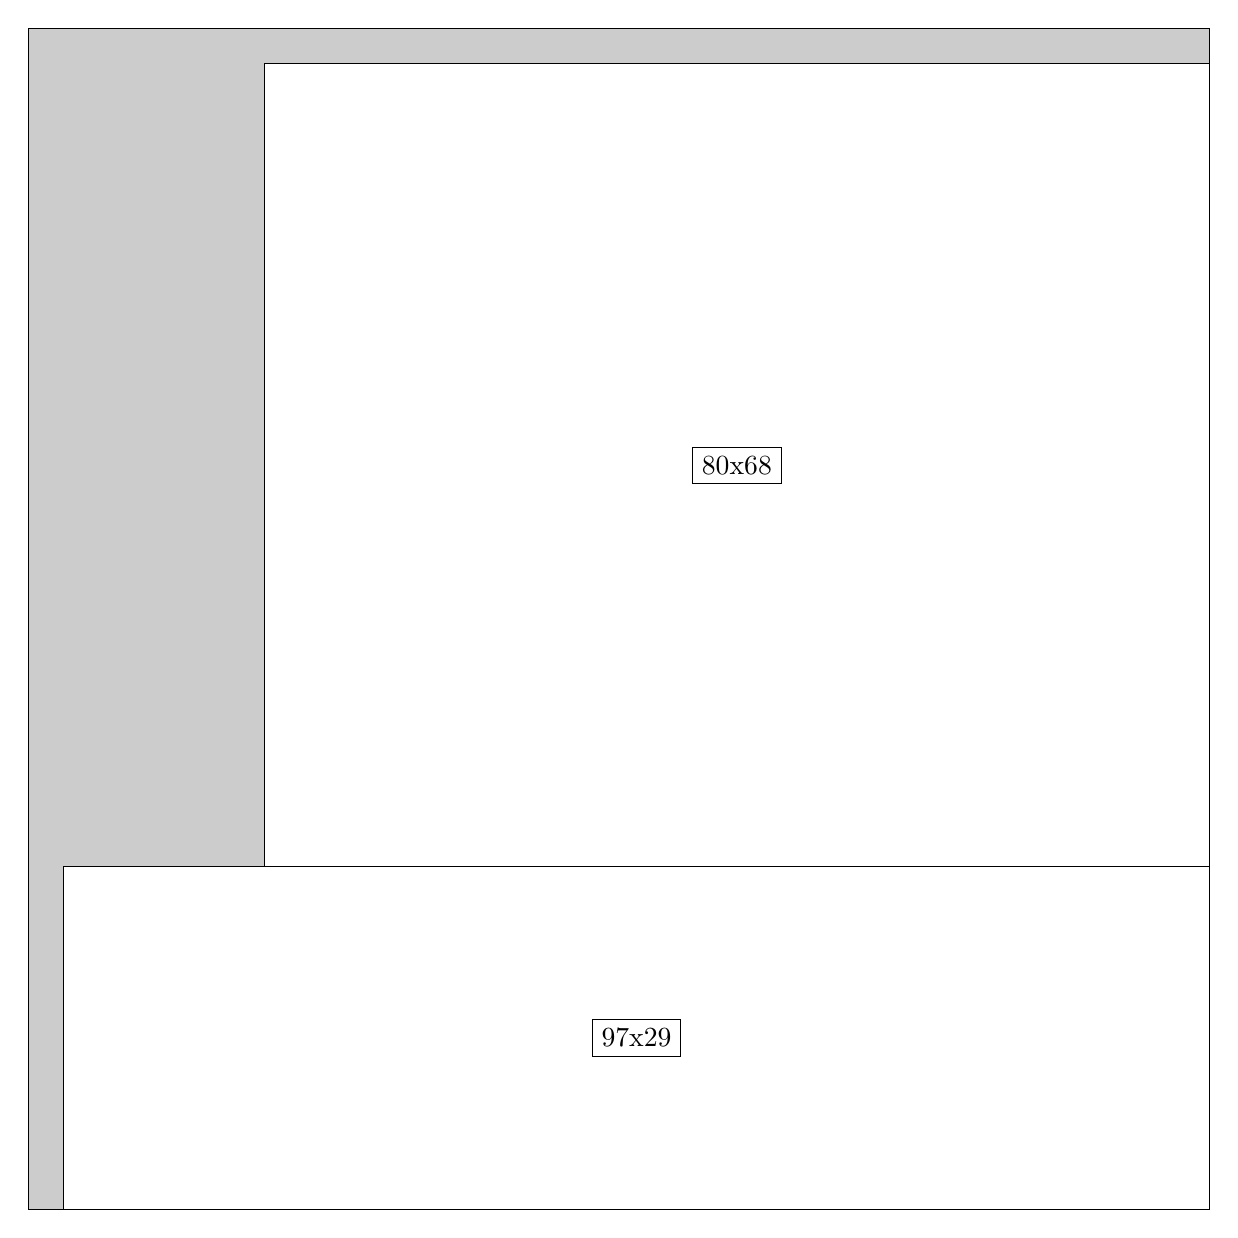
\begin{tikzpicture}[shorten >=1pt,scale=1.0,every node/.style={scale=1.0},->]
\tikzstyle{vertex}=[circle,fill=black!25,minimum size=14pt,inner sep=0pt]
\filldraw[fill=gray!40!white, draw=black] (0,0) rectangle (15.0,15.0);
\foreach \name/\x/\y/\w/\h in {97x29/0.44999999999999996/0.0/14.549999999999999/4.35,80x68/3.0/4.35/12.0/10.2}
\filldraw[fill=white!40!white, draw=black] (\x,\y) rectangle node[draw] (\name) {\name} ++(\w,\h);
\end{tikzpicture}


w =97 , h =29 , x =3 , y =0 , v =2813
\par
w =80 , h =68 , x =20 , y =29 , v =5440
\par
\newpage


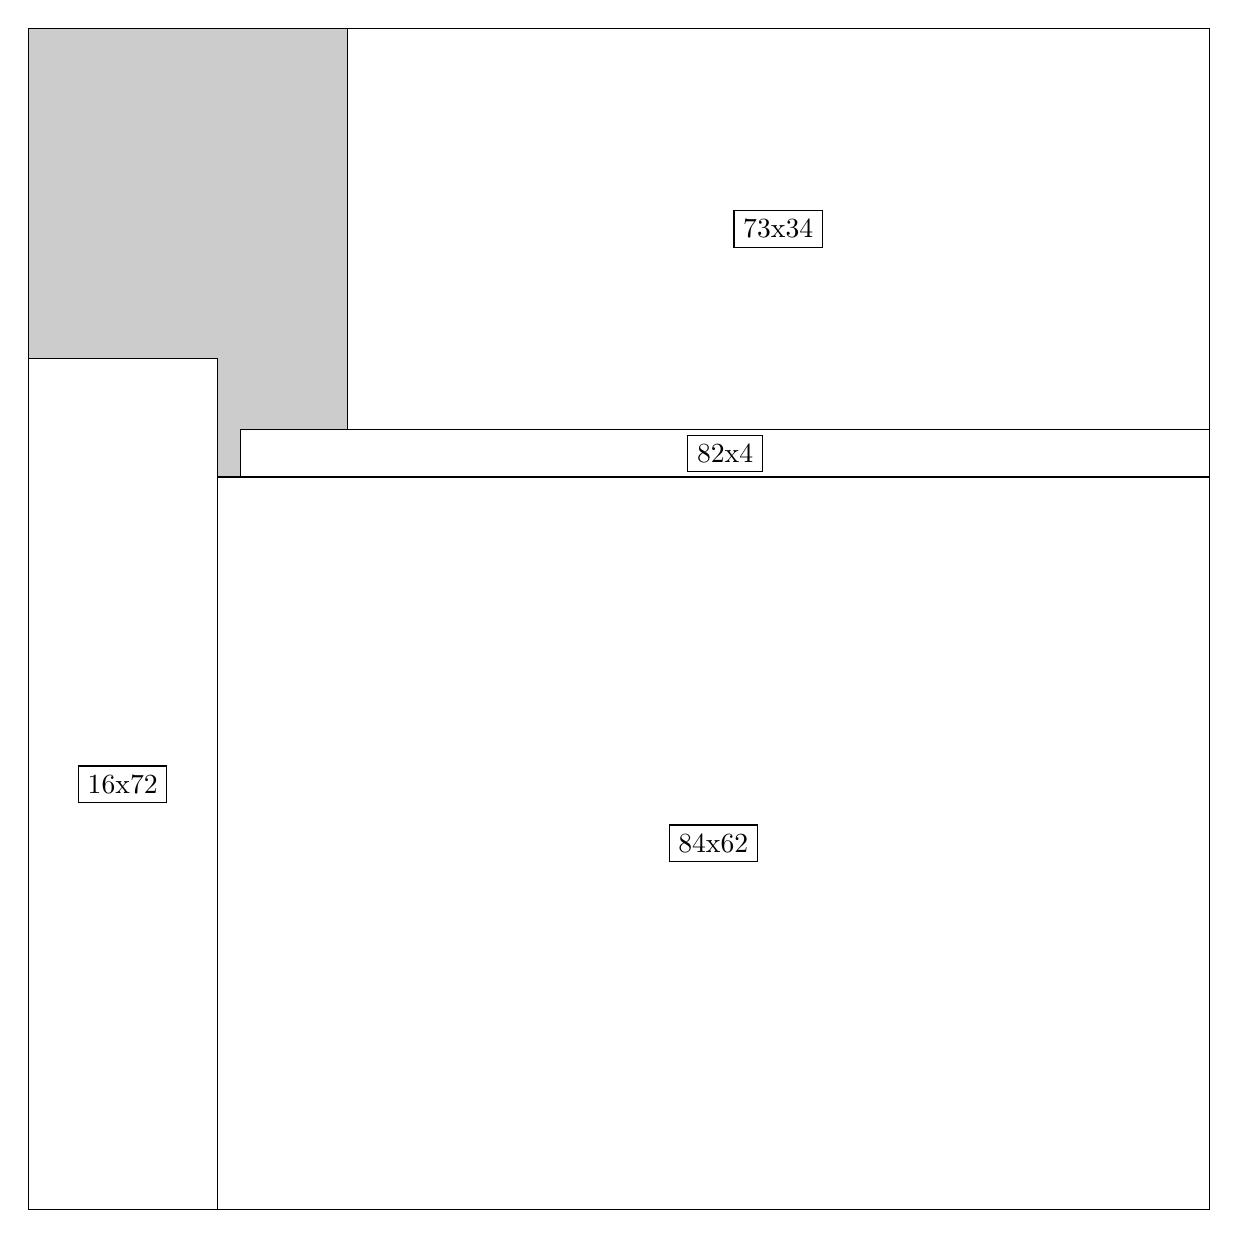
\begin{tikzpicture}[shorten >=1pt,scale=1.0,every node/.style={scale=1.0},->]
\tikzstyle{vertex}=[circle,fill=black!25,minimum size=14pt,inner sep=0pt]
\filldraw[fill=gray!40!white, draw=black] (0,0) rectangle (15.0,15.0);
\foreach \name/\x/\y/\w/\h in {84x62/2.4/0.0/12.6/9.299999999999999,82x4/2.6999999999999997/9.299999999999999/12.299999999999999/0.6,73x34/4.05/9.9/10.95/5.1,16x72/0.0/0.0/2.4/10.799999999999999}
\filldraw[fill=white!40!white, draw=black] (\x,\y) rectangle node[draw] (\name) {\name} ++(\w,\h);
\end{tikzpicture}


w =84 , h =62 , x =16 , y =0 , v =5208
\par
w =82 , h =4 , x =18 , y =62 , v =328
\par
w =73 , h =34 , x =27 , y =66 , v =2482
\par
w =16 , h =72 , x =0 , y =0 , v =1152
\par
\newpage


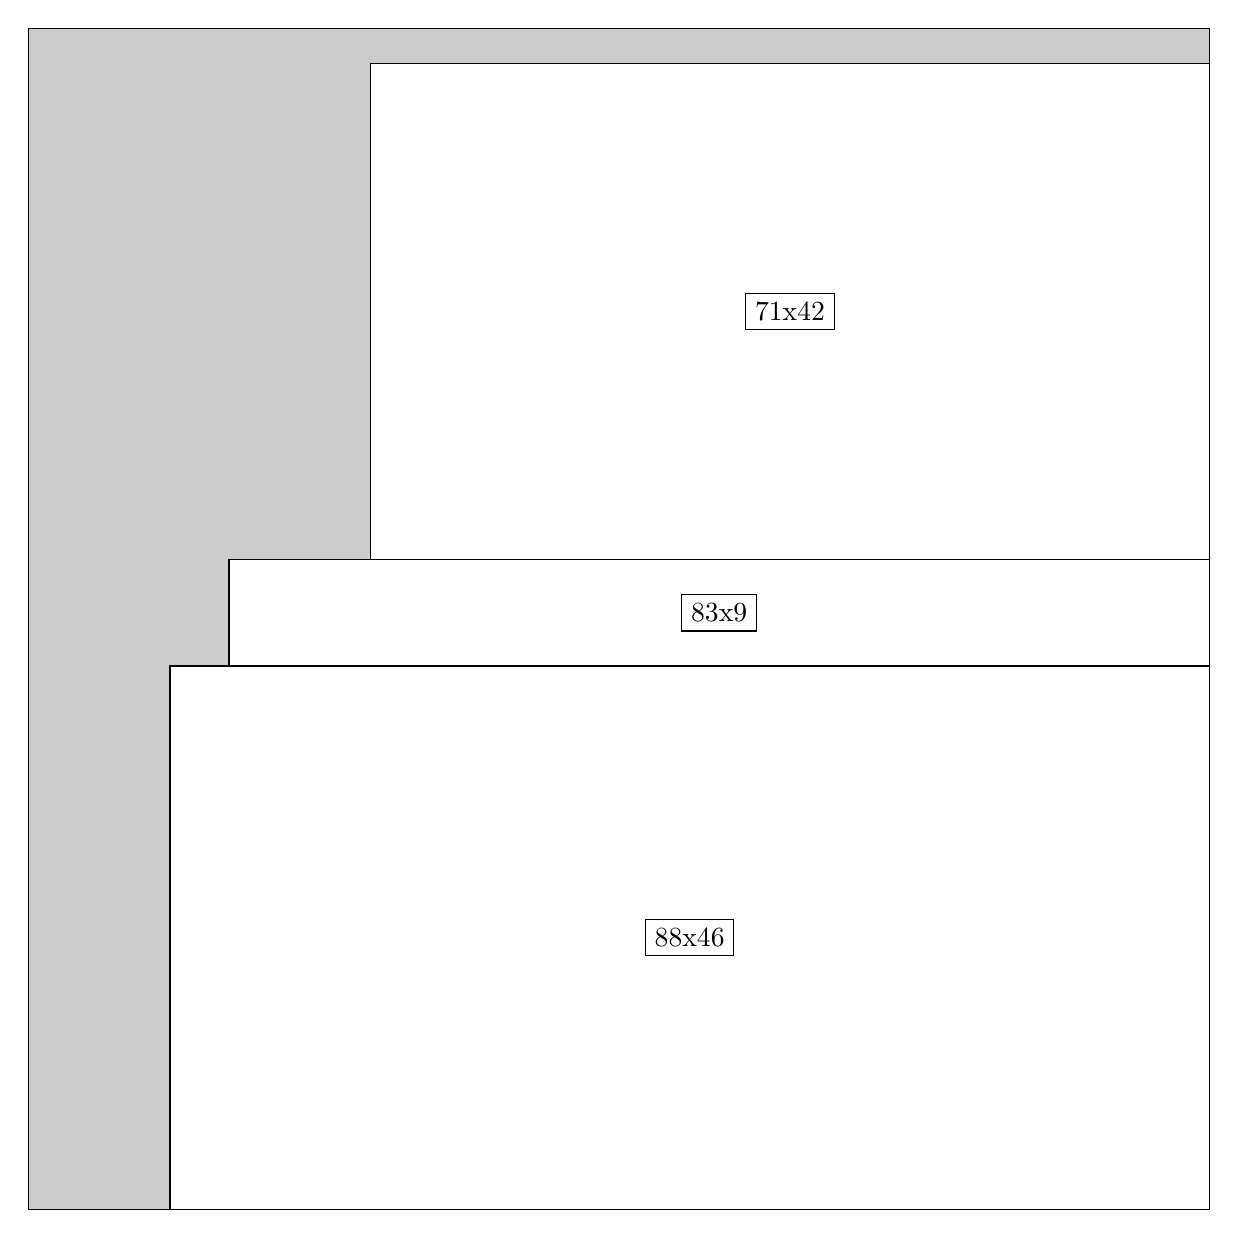
\begin{tikzpicture}[shorten >=1pt,scale=1.0,every node/.style={scale=1.0},->]
\tikzstyle{vertex}=[circle,fill=black!25,minimum size=14pt,inner sep=0pt]
\filldraw[fill=gray!40!white, draw=black] (0,0) rectangle (15.0,15.0);
\foreach \name/\x/\y/\w/\h in {88x46/1.7999999999999998/0.0/13.2/6.8999999999999995,83x9/2.55/6.8999999999999995/12.45/1.3499999999999999,71x42/4.35/8.25/10.65/6.3}
\filldraw[fill=white!40!white, draw=black] (\x,\y) rectangle node[draw] (\name) {\name} ++(\w,\h);
\end{tikzpicture}


w =88 , h =46 , x =12 , y =0 , v =4048
\par
w =83 , h =9 , x =17 , y =46 , v =747
\par
w =71 , h =42 , x =29 , y =55 , v =2982
\par
\newpage


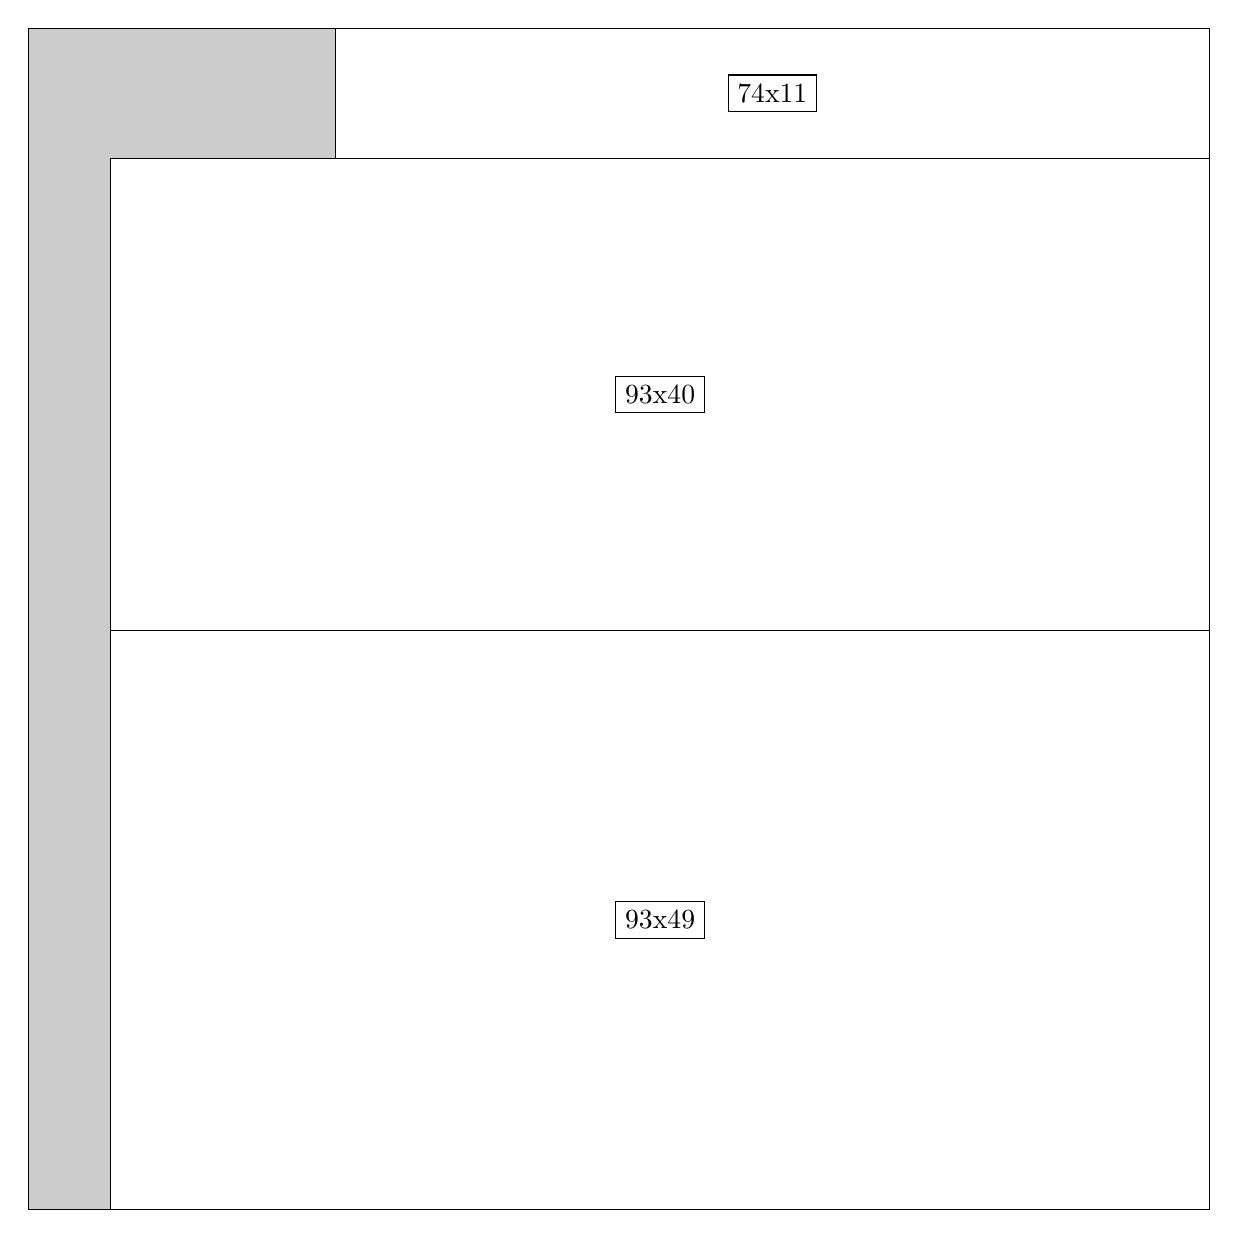
\begin{tikzpicture}[shorten >=1pt,scale=1.0,every node/.style={scale=1.0},->]
\tikzstyle{vertex}=[circle,fill=black!25,minimum size=14pt,inner sep=0pt]
\filldraw[fill=gray!40!white, draw=black] (0,0) rectangle (15.0,15.0);
\foreach \name/\x/\y/\w/\h in {93x49/1.05/0.0/13.95/7.35,93x40/1.05/7.35/13.95/6.0,74x11/3.9/13.35/11.1/1.65}
\filldraw[fill=white!40!white, draw=black] (\x,\y) rectangle node[draw] (\name) {\name} ++(\w,\h);
\end{tikzpicture}


w =93 , h =49 , x =7 , y =0 , v =4557
\par
w =93 , h =40 , x =7 , y =49 , v =3720
\par
w =74 , h =11 , x =26 , y =89 , v =814
\par
\newpage


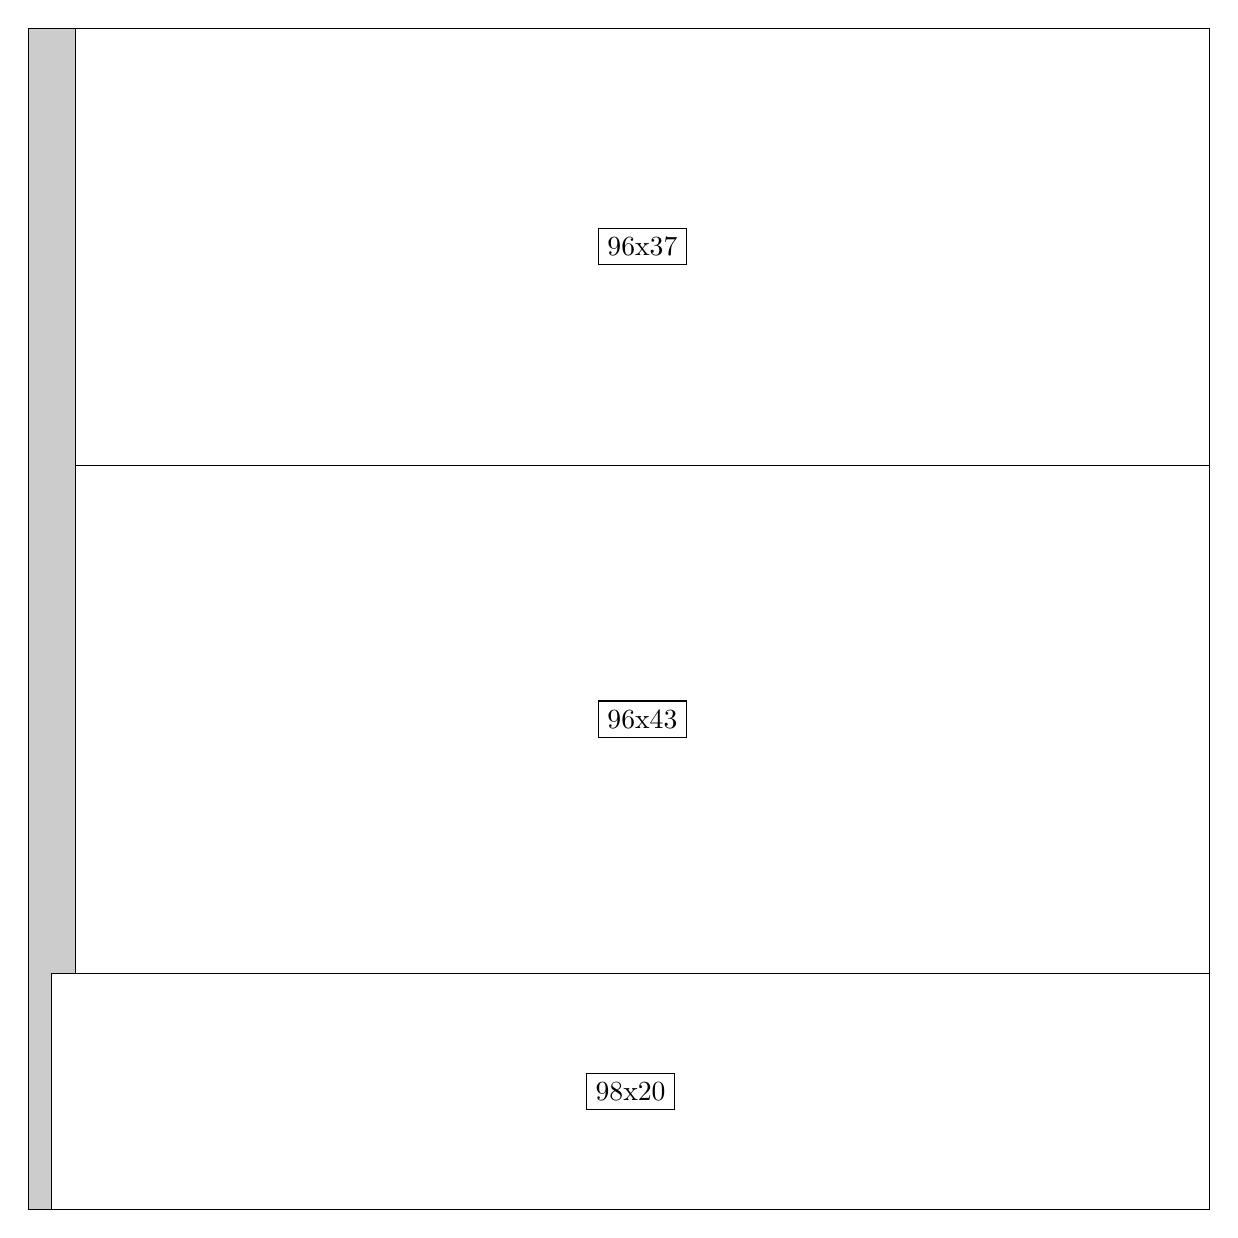
\begin{tikzpicture}[shorten >=1pt,scale=1.0,every node/.style={scale=1.0},->]
\tikzstyle{vertex}=[circle,fill=black!25,minimum size=14pt,inner sep=0pt]
\filldraw[fill=gray!40!white, draw=black] (0,0) rectangle (15.0,15.0);
\foreach \name/\x/\y/\w/\h in {98x20/0.3/0.0/14.7/3.0,96x43/0.6/3.0/14.399999999999999/6.45,96x37/0.6/9.45/14.399999999999999/5.55}
\filldraw[fill=white!40!white, draw=black] (\x,\y) rectangle node[draw] (\name) {\name} ++(\w,\h);
\end{tikzpicture}


w =98 , h =20 , x =2 , y =0 , v =1960
\par
w =96 , h =43 , x =4 , y =20 , v =4128
\par
w =96 , h =37 , x =4 , y =63 , v =3552
\par
\newpage


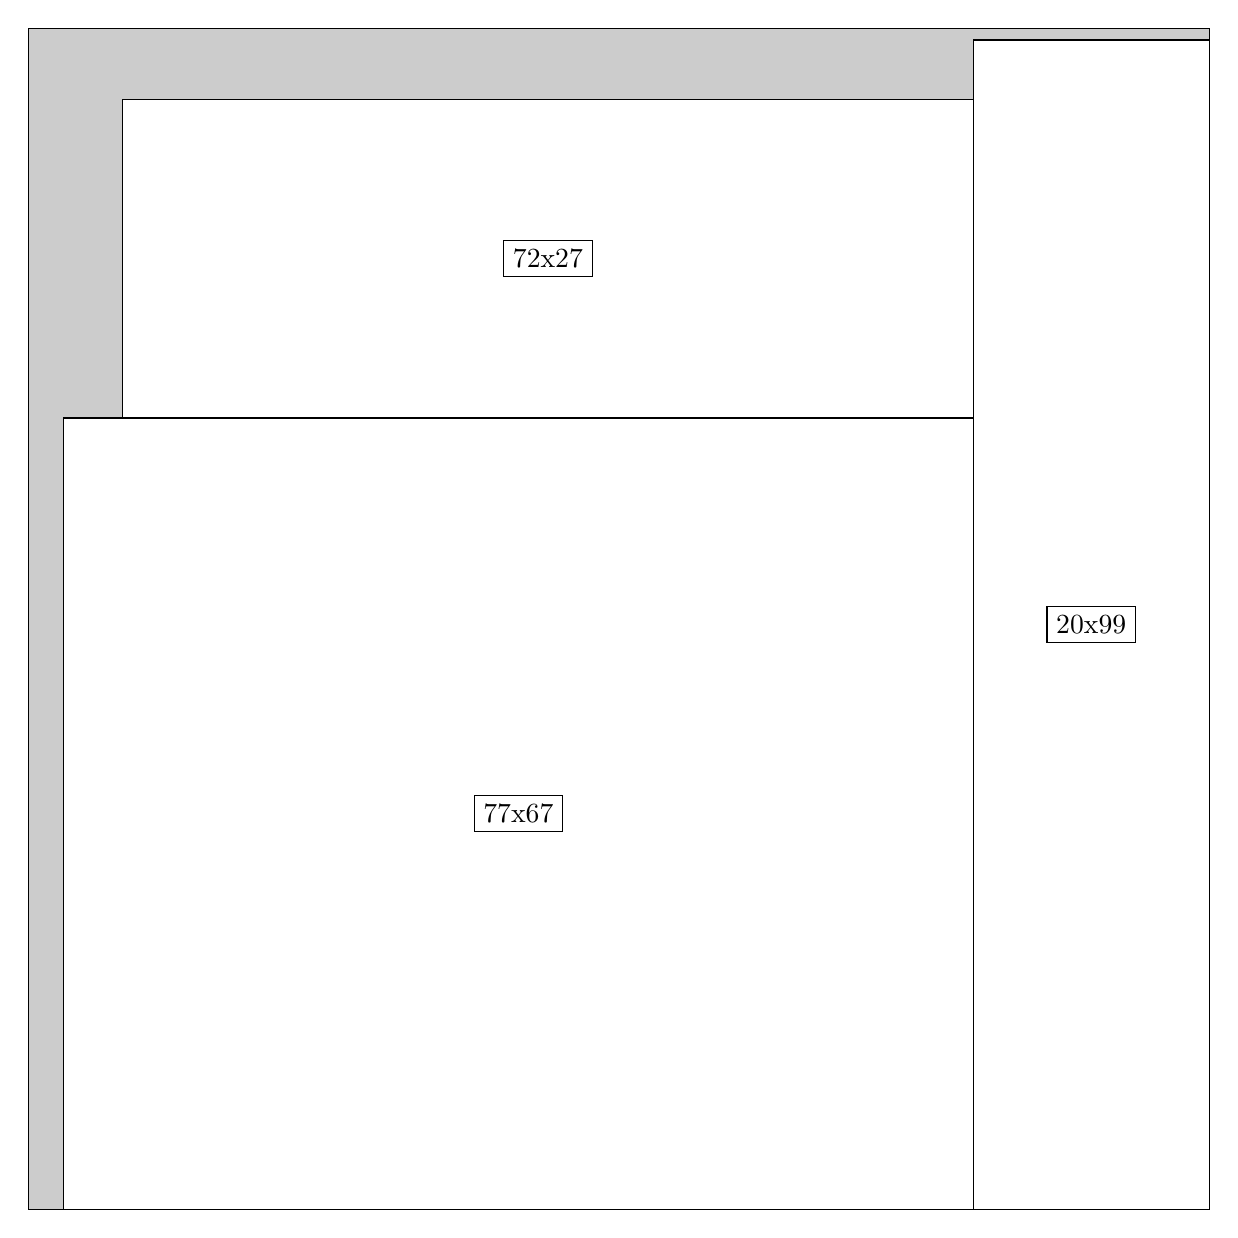
\begin{tikzpicture}[shorten >=1pt,scale=1.0,every node/.style={scale=1.0},->]
\tikzstyle{vertex}=[circle,fill=black!25,minimum size=14pt,inner sep=0pt]
\filldraw[fill=gray!40!white, draw=black] (0,0) rectangle (15.0,15.0);
\foreach \name/\x/\y/\w/\h in {20x99/12.0/0.0/3.0/14.85,77x67/0.44999999999999996/0.0/11.549999999999999/10.049999999999999,72x27/1.2/10.049999999999999/10.799999999999999/4.05}
\filldraw[fill=white!40!white, draw=black] (\x,\y) rectangle node[draw] (\name) {\name} ++(\w,\h);
\end{tikzpicture}


w =20 , h =99 , x =80 , y =0 , v =1980
\par
w =77 , h =67 , x =3 , y =0 , v =5159
\par
w =72 , h =27 , x =8 , y =67 , v =1944
\par
\newpage


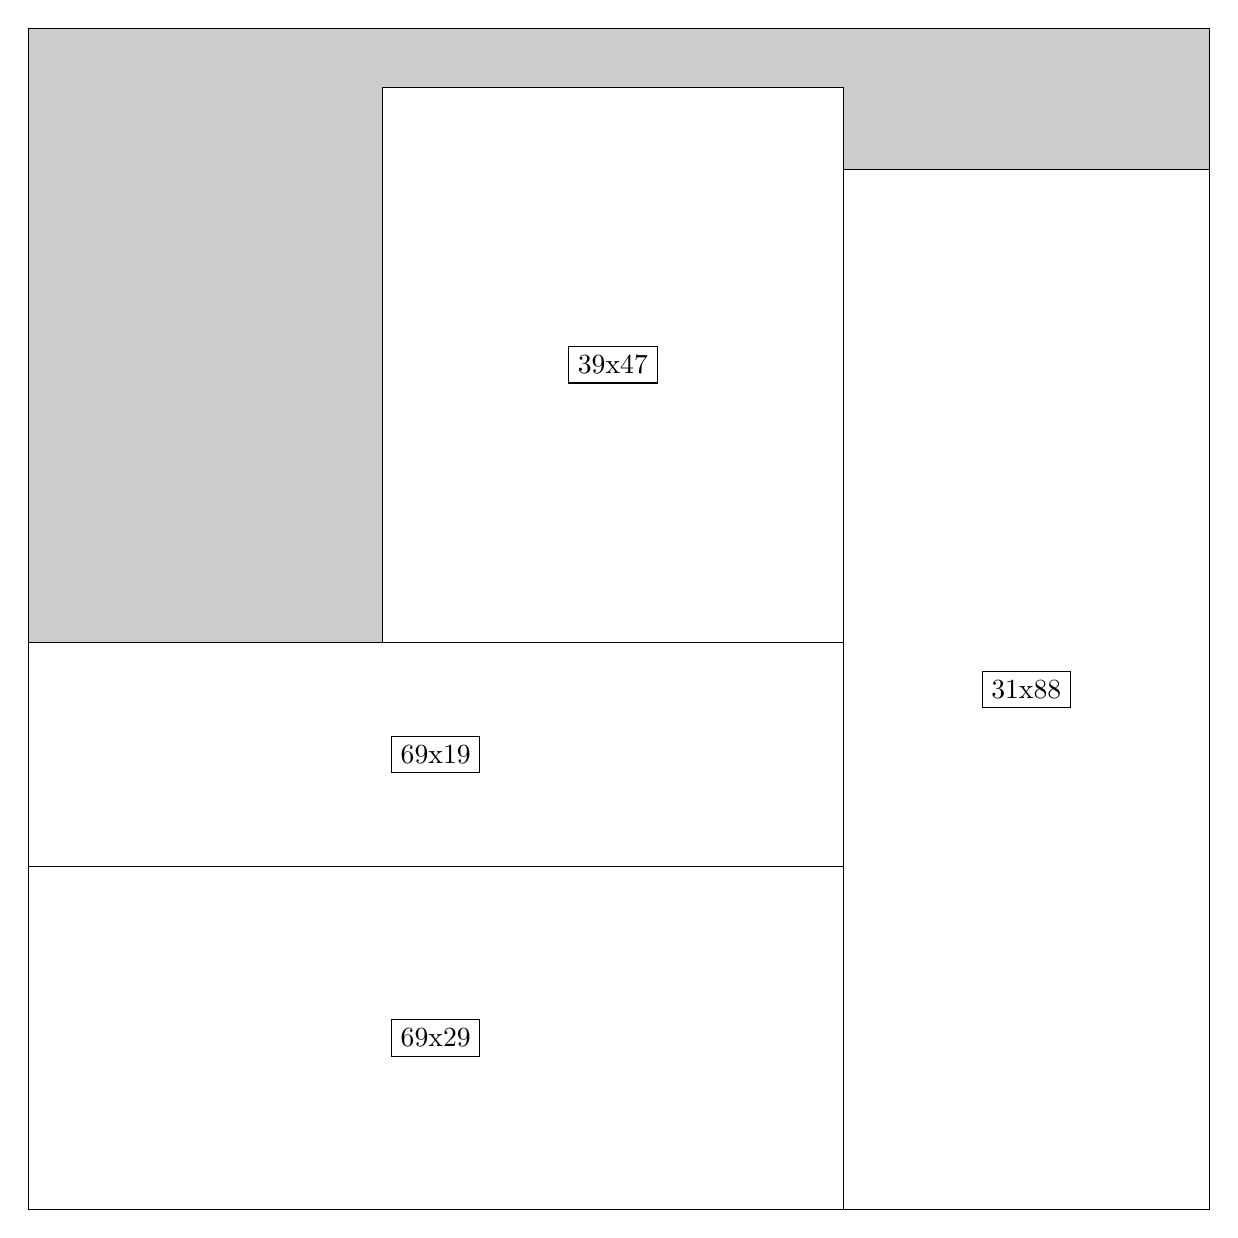
\begin{tikzpicture}[shorten >=1pt,scale=1.0,every node/.style={scale=1.0},->]
\tikzstyle{vertex}=[circle,fill=black!25,minimum size=14pt,inner sep=0pt]
\filldraw[fill=gray!40!white, draw=black] (0,0) rectangle (15.0,15.0);
\foreach \name/\x/\y/\w/\h in {31x88/10.35/0.0/4.6499999999999995/13.2,69x29/0.0/0.0/10.35/4.35,69x19/0.0/4.35/10.35/2.85,39x47/4.5/7.199999999999999/5.85/7.05}
\filldraw[fill=white!40!white, draw=black] (\x,\y) rectangle node[draw] (\name) {\name} ++(\w,\h);
\end{tikzpicture}


w =31 , h =88 , x =69 , y =0 , v =2728
\par
w =69 , h =29 , x =0 , y =0 , v =2001
\par
w =69 , h =19 , x =0 , y =29 , v =1311
\par
w =39 , h =47 , x =30 , y =48 , v =1833
\par
\newpage


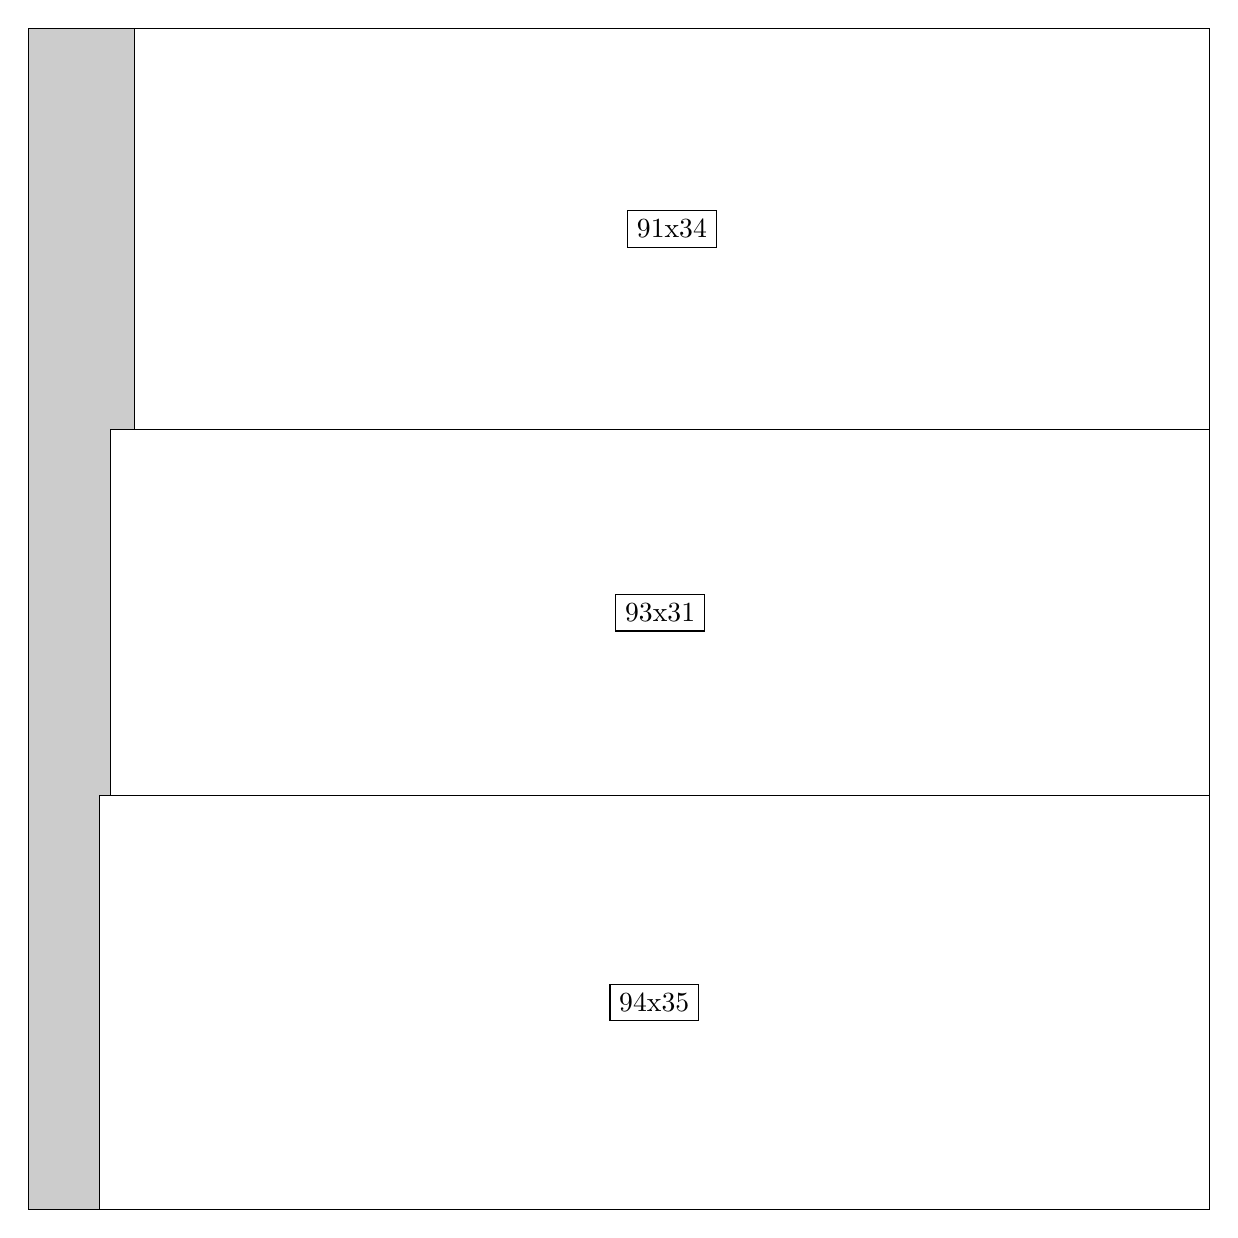
\begin{tikzpicture}[shorten >=1pt,scale=1.0,every node/.style={scale=1.0},->]
\tikzstyle{vertex}=[circle,fill=black!25,minimum size=14pt,inner sep=0pt]
\filldraw[fill=gray!40!white, draw=black] (0,0) rectangle (15.0,15.0);
\foreach \name/\x/\y/\w/\h in {94x35/0.8999999999999999/0.0/14.1/5.25,93x31/1.05/5.25/13.95/4.6499999999999995,91x34/1.3499999999999999/9.9/13.65/5.1}
\filldraw[fill=white!40!white, draw=black] (\x,\y) rectangle node[draw] (\name) {\name} ++(\w,\h);
\end{tikzpicture}


w =94 , h =35 , x =6 , y =0 , v =3290
\par
w =93 , h =31 , x =7 , y =35 , v =2883
\par
w =91 , h =34 , x =9 , y =66 , v =3094
\par
\newpage


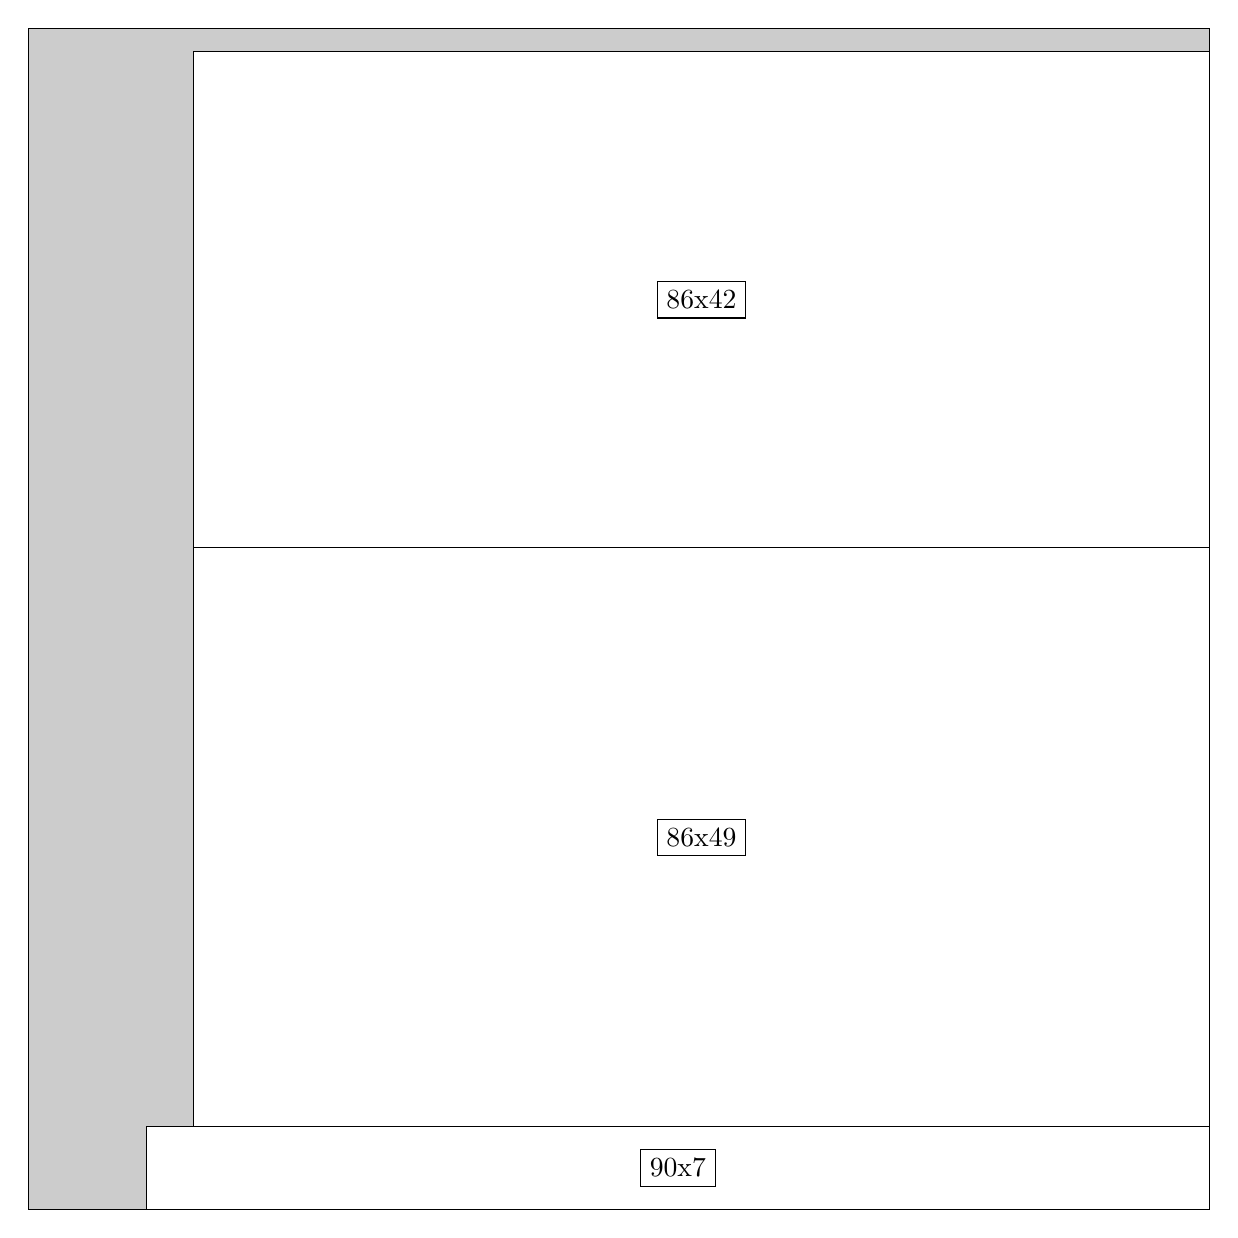
\begin{tikzpicture}[shorten >=1pt,scale=1.0,every node/.style={scale=1.0},->]
\tikzstyle{vertex}=[circle,fill=black!25,minimum size=14pt,inner sep=0pt]
\filldraw[fill=gray!40!white, draw=black] (0,0) rectangle (15.0,15.0);
\foreach \name/\x/\y/\w/\h in {90x7/1.5/0.0/13.5/1.05,86x49/2.1/1.05/12.9/7.35,86x42/2.1/8.4/12.9/6.3}
\filldraw[fill=white!40!white, draw=black] (\x,\y) rectangle node[draw] (\name) {\name} ++(\w,\h);
\end{tikzpicture}


w =90 , h =7 , x =10 , y =0 , v =630
\par
w =86 , h =49 , x =14 , y =7 , v =4214
\par
w =86 , h =42 , x =14 , y =56 , v =3612
\par
\newpage


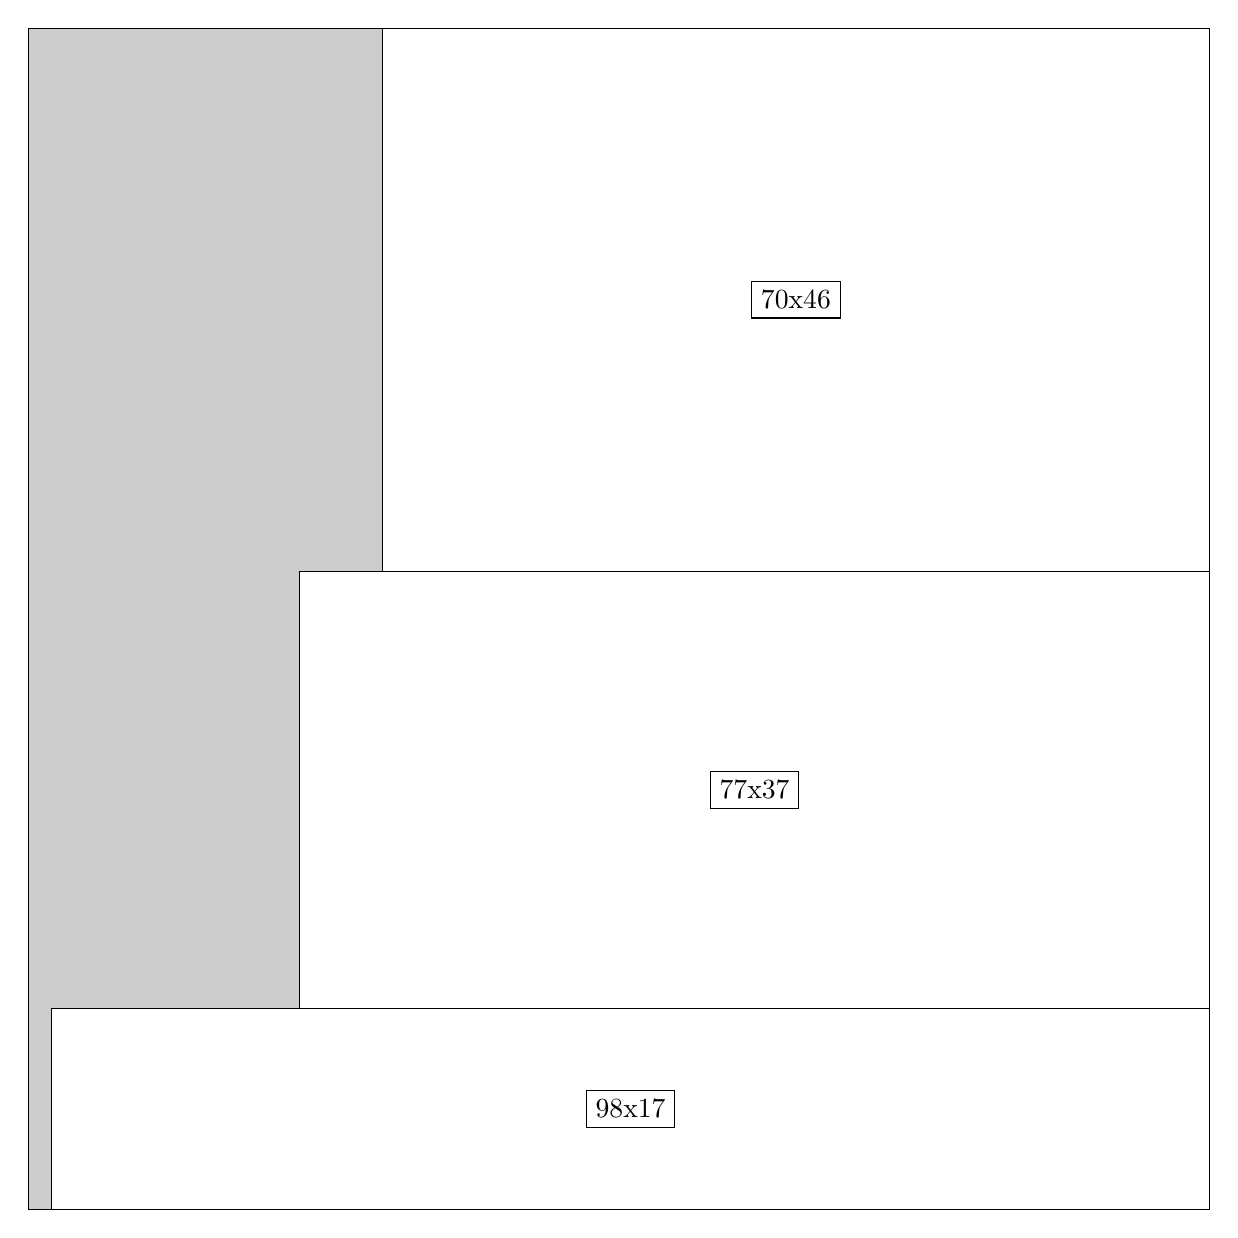
\begin{tikzpicture}[shorten >=1pt,scale=1.0,every node/.style={scale=1.0},->]
\tikzstyle{vertex}=[circle,fill=black!25,minimum size=14pt,inner sep=0pt]
\filldraw[fill=gray!40!white, draw=black] (0,0) rectangle (15.0,15.0);
\foreach \name/\x/\y/\w/\h in {98x17/0.3/0.0/14.7/2.55,77x37/3.4499999999999997/2.55/11.549999999999999/5.55,70x46/4.5/8.1/10.5/6.8999999999999995}
\filldraw[fill=white!40!white, draw=black] (\x,\y) rectangle node[draw] (\name) {\name} ++(\w,\h);
\end{tikzpicture}


w =98 , h =17 , x =2 , y =0 , v =1666
\par
w =77 , h =37 , x =23 , y =17 , v =2849
\par
w =70 , h =46 , x =30 , y =54 , v =3220
\par
\newpage


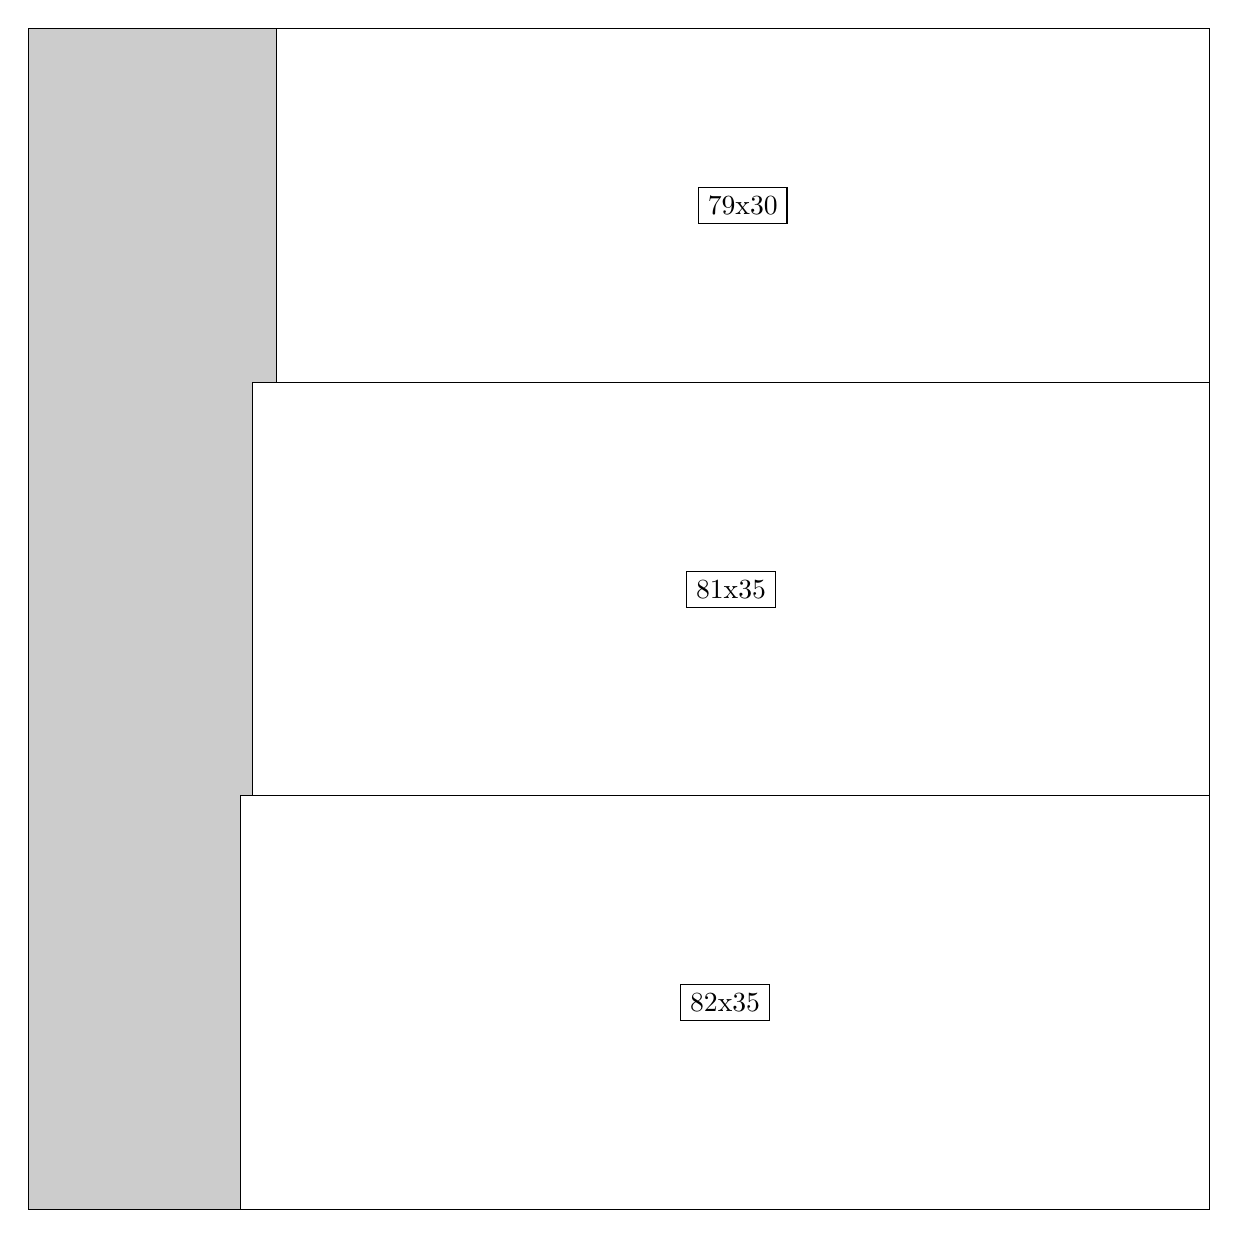
\begin{tikzpicture}[shorten >=1pt,scale=1.0,every node/.style={scale=1.0},->]
\tikzstyle{vertex}=[circle,fill=black!25,minimum size=14pt,inner sep=0pt]
\filldraw[fill=gray!40!white, draw=black] (0,0) rectangle (15.0,15.0);
\foreach \name/\x/\y/\w/\h in {82x35/2.6999999999999997/0.0/12.299999999999999/5.25,81x35/2.85/5.25/12.15/5.25,79x30/3.15/10.5/11.85/4.5}
\filldraw[fill=white!40!white, draw=black] (\x,\y) rectangle node[draw] (\name) {\name} ++(\w,\h);
\end{tikzpicture}


w =82 , h =35 , x =18 , y =0 , v =2870
\par
w =81 , h =35 , x =19 , y =35 , v =2835
\par
w =79 , h =30 , x =21 , y =70 , v =2370
\par
\newpage


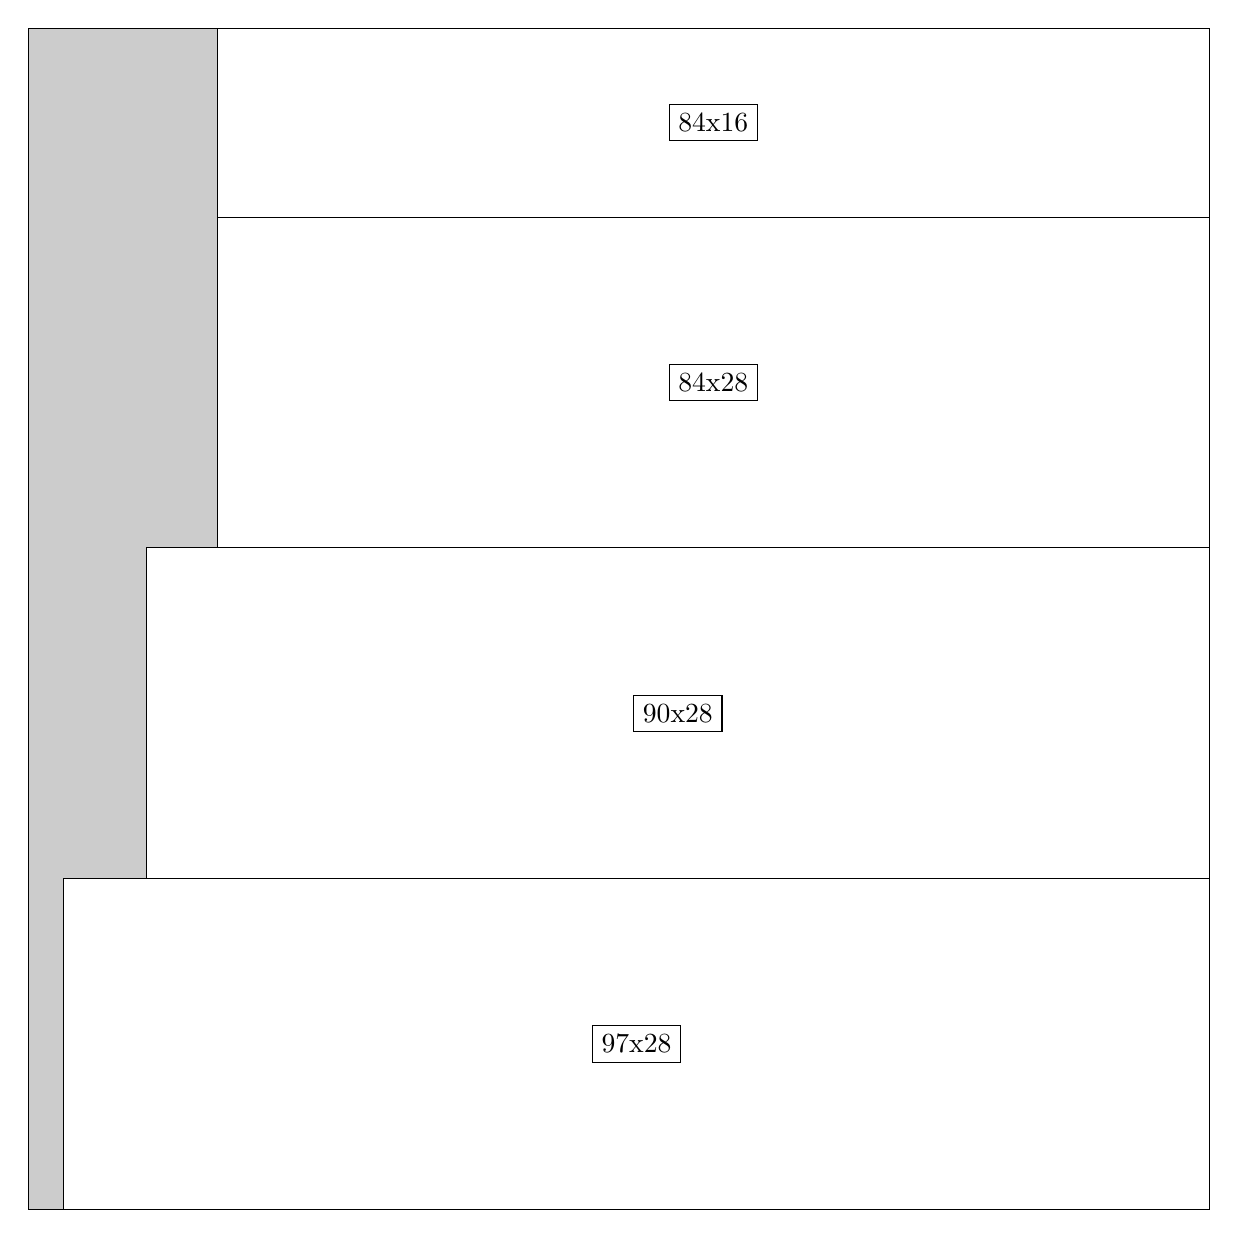
\begin{tikzpicture}[shorten >=1pt,scale=1.0,every node/.style={scale=1.0},->]
\tikzstyle{vertex}=[circle,fill=black!25,minimum size=14pt,inner sep=0pt]
\filldraw[fill=gray!40!white, draw=black] (0,0) rectangle (15.0,15.0);
\foreach \name/\x/\y/\w/\h in {97x28/0.44999999999999996/0.0/14.549999999999999/4.2,90x28/1.5/4.2/13.5/4.2,84x28/2.4/8.4/12.6/4.2,84x16/2.4/12.6/12.6/2.4}
\filldraw[fill=white!40!white, draw=black] (\x,\y) rectangle node[draw] (\name) {\name} ++(\w,\h);
\end{tikzpicture}


w =97 , h =28 , x =3 , y =0 , v =2716
\par
w =90 , h =28 , x =10 , y =28 , v =2520
\par
w =84 , h =28 , x =16 , y =56 , v =2352
\par
w =84 , h =16 , x =16 , y =84 , v =1344
\par
\newpage


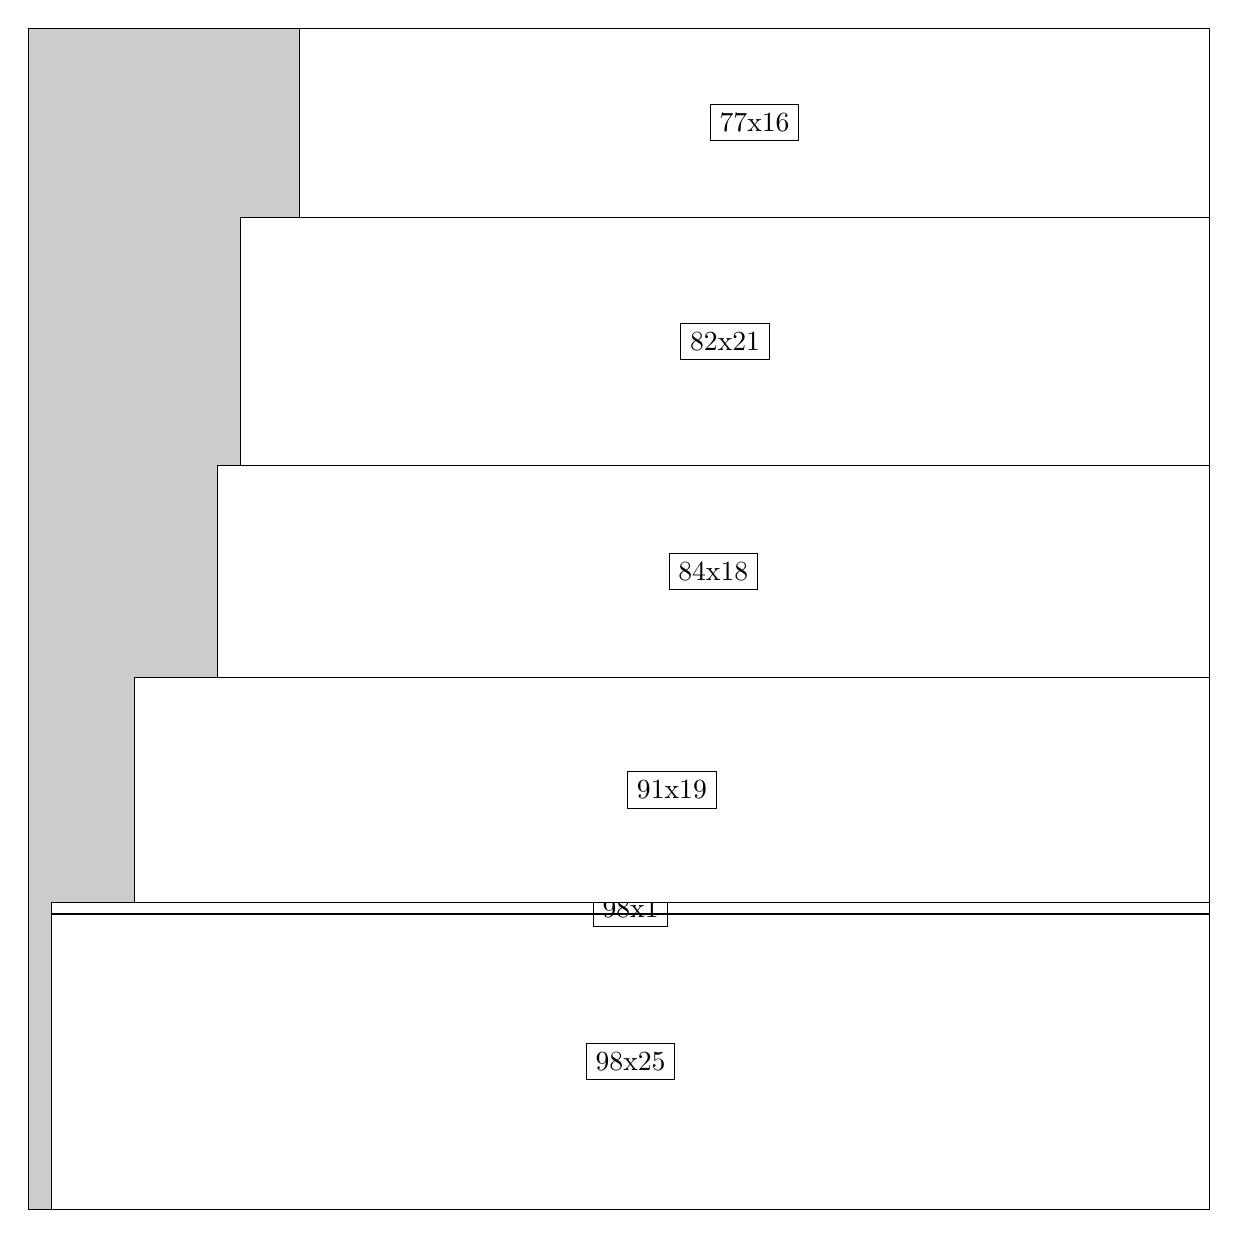
\begin{tikzpicture}[shorten >=1pt,scale=1.0,every node/.style={scale=1.0},->]
\tikzstyle{vertex}=[circle,fill=black!25,minimum size=14pt,inner sep=0pt]
\filldraw[fill=gray!40!white, draw=black] (0,0) rectangle (15.0,15.0);
\foreach \name/\x/\y/\w/\h in {98x25/0.3/0.0/14.7/3.75,98x1/0.3/3.75/14.7/0.15,91x19/1.3499999999999999/3.9/13.65/2.85,84x18/2.4/6.75/12.6/2.6999999999999997,82x21/2.6999999999999997/9.45/12.299999999999999/3.15,77x16/3.4499999999999997/12.6/11.549999999999999/2.4}
\filldraw[fill=white!40!white, draw=black] (\x,\y) rectangle node[draw] (\name) {\name} ++(\w,\h);
\end{tikzpicture}


w =98 , h =25 , x =2 , y =0 , v =2450
\par
w =98 , h =1 , x =2 , y =25 , v =98
\par
w =91 , h =19 , x =9 , y =26 , v =1729
\par
w =84 , h =18 , x =16 , y =45 , v =1512
\par
w =82 , h =21 , x =18 , y =63 , v =1722
\par
w =77 , h =16 , x =23 , y =84 , v =1232
\par
\newpage


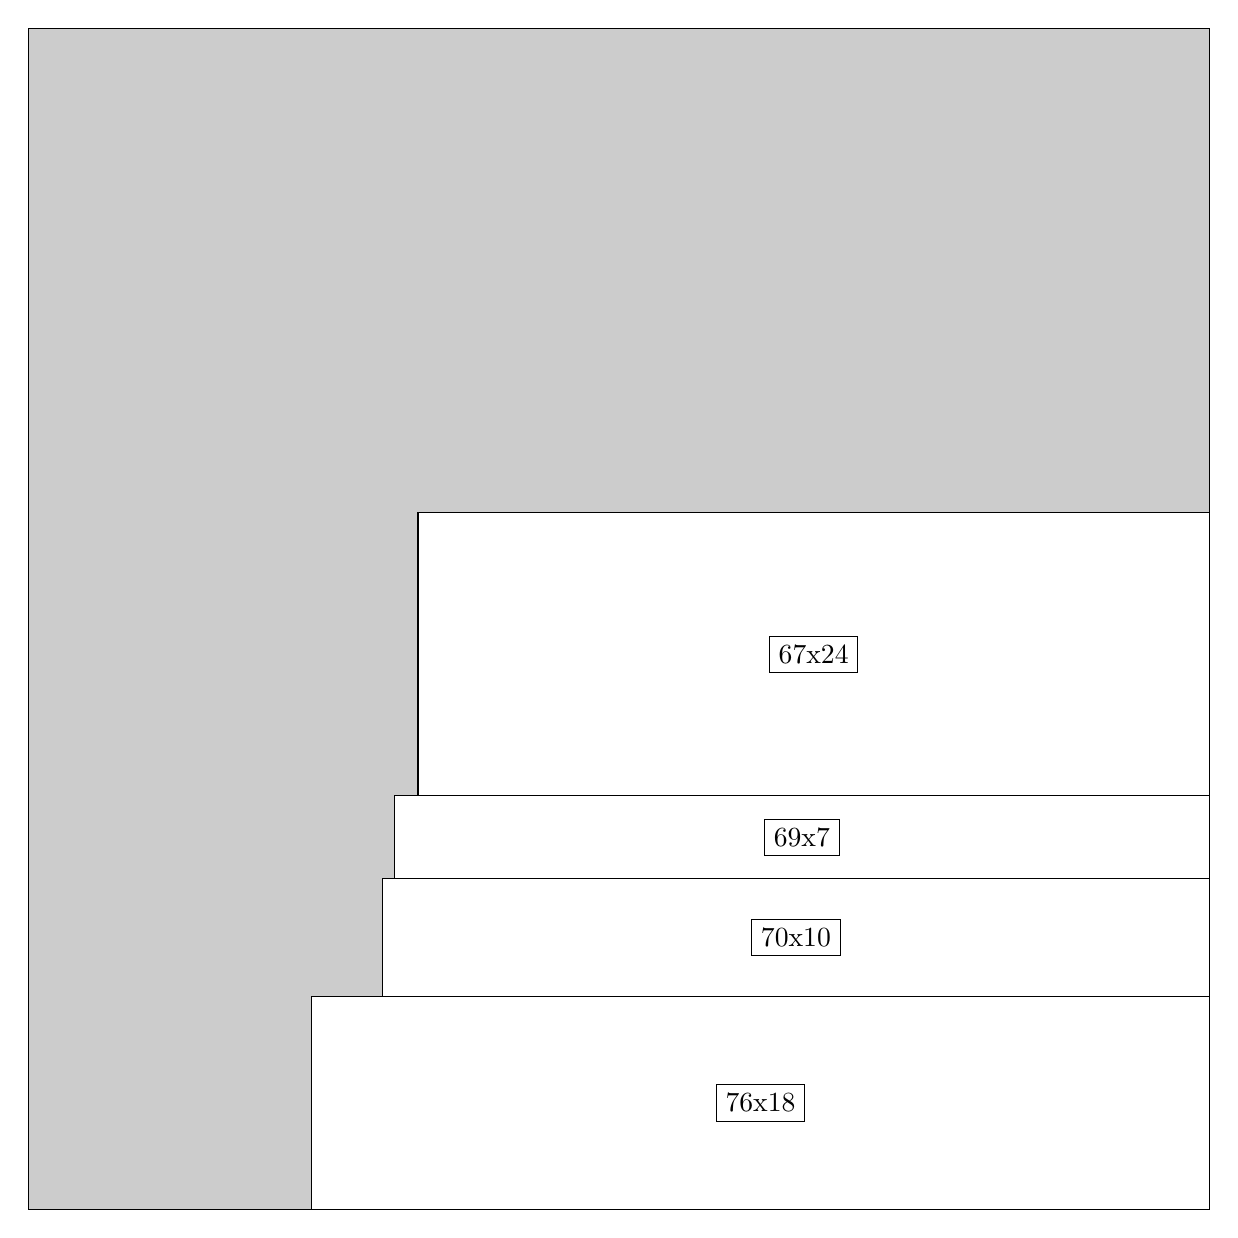
\begin{tikzpicture}[shorten >=1pt,scale=1.0,every node/.style={scale=1.0},->]
\tikzstyle{vertex}=[circle,fill=black!25,minimum size=14pt,inner sep=0pt]
\filldraw[fill=gray!40!white, draw=black] (0,0) rectangle (15.0,15.0);
\foreach \name/\x/\y/\w/\h in {76x18/3.5999999999999996/0.0/11.4/2.6999999999999997,70x10/4.5/2.6999999999999997/10.5/1.5,69x7/4.6499999999999995/4.2/10.35/1.05,67x24/4.95/5.25/10.049999999999999/3.5999999999999996}
\filldraw[fill=white!40!white, draw=black] (\x,\y) rectangle node[draw] (\name) {\name} ++(\w,\h);
\end{tikzpicture}


w =76 , h =18 , x =24 , y =0 , v =1368
\par
w =70 , h =10 , x =30 , y =18 , v =700
\par
w =69 , h =7 , x =31 , y =28 , v =483
\par
w =67 , h =24 , x =33 , y =35 , v =1608
\par
\newpage


\end{document}